%%%%%%%%%%%%%%%%%%%%%%%%%%%%%%%%
% INCLUSION PREAMBULE COMMUN   %
%%%%%%%%%%%%%%%%%%%%%%%%%%%%%%%%
% définition et packages du présent fichier
%%%%%%%%%%%%%%%%%%%%%%%%%
% PACKAGES              %
%%%%%%%%%%%%%%%%%%%%%%%%%
\documentclass{report}
\usepackage[utf8x]{inputenc}  % accents
\usepackage{geometry}         % marges
\usepackage[francais]{babel}  % langue
\usepackage{graphicx}         % images
\usepackage{verbatim}         % texte préformaté
\usepackage{fancyhdr}         % fancy






% Titre de ce fichier dans le fancy 
\newcommand{\titre}{{\Huge Manuel d'utilisation}\\de Picross} 
\newcommand{\titrehead}{Manuel d'utilisation}
    
% Inclusion du préambule commun
%%%%%%%%%%%%%%%%%%%%%%%%%
% PRÉAMBULE             %
%%%%%%%%%%%%%%%%%%%%%%%%%
\title{\titre{}}
\author{}
% laisser vide pour date de compilation
\date{} 

% FORMAT PAGES         
\pagestyle{fancy} % nom du rendu (définit les lignes suivantes)
        \lhead{} % left head
        \chead{\titrehead{}} % center head
        \rhead{} % right head
        \lfoot{} % left foot
        \cfoot{\thepage} % center foot
        \rfoot{} % right foot


% Ce fichier est un préambule commun à toutes les sources LaTeX.
% Il est inclus par toutes les sources et permet d'avoir un formatage commun facilement modifiable.


%

%%%%%%%%%%%%%%%%%%%%%%%%%
% BEGIN                 %
%%%%%%%%%%%%%%%%%%%%%%%%%
\begin{document}
\maketitle
\tableofcontents




\chapter{Picross}
\section{Principe du Jeu}
        \paragraph*{}
       Le but consiste à noircir les cases selon les chiffres indiqués de part et d'autre de la grille. Ils indiquent la taille des blocs de cases noires de la ligne ou de la colonne sur laquelle ils se trouvent.\\ 

       \begin{center}
                      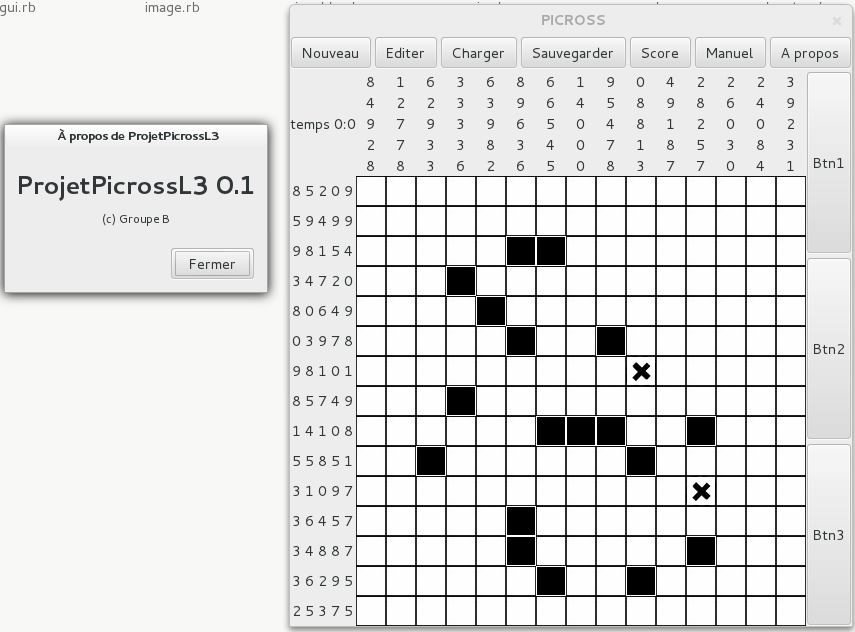
\includegraphics[scale=0.6]{data/screenMaquette/APropos.png}\\
                      \textbf{Picross interface}
      \end{center}

\section{Régle du jeu}
        \paragraph*{}
        Par exemple 3,4 à gauche d’une ligne indique qu’il y a, de gauche à droite,
un bloc de 3 cases consécutive noires puis un bloc de 4 cases consécutive noires
sur cette ligne. En revanche, ce qui n’est pas mentionné et qui fait la difficulté,
est le nombre de cases blanches entre les cases noires. On sait simplement qu’il
y en a au moins une. Chaque grille résolue fait découvrir un dessin. Trouver les
cellules vides est aussi important que de trouver les cellules noires, car, plus tard,
les cellules vides permettront de décider où se situera un bloc de cellules noires.\\ 
On marque généralement une cellule vide par une croix, ou drapeau, afin de différencier les cases vides et les cases dont l'état final n'a pas encore été trouvé.


\section{Les différents types de clic pour une case}
        \paragraph*{}
        \begin{itemize}
                \item noircir une case : clic gauche (souris) ;
                \item noircir plusieurs cases : clic gauche (souris), maintenir et glisser jusqu’à la case voulue, relâcher (uniquement dans le mode multiple). ;
                \item éliminer une case : clic droit (souris) ;
                \item éliminer plusieurs cases : clic droit (souris), maintenir et glisser jusqu’à la case voulue, relâcher ; \\ \\             
        \end{itemize}





\section{Menu}
        \paragraph*{}
        Le menu contient les fonctionnalités suivantes : Nouvelle grille, Editer une grille, Charger une grille, Sauvegarder la grille courante, Score, Manuel d'aide, Préférences, A Propos \\
        
               \begin{center}
                      
\includegraphics[scale=0.6]{data/screenMaquette/menu.png}\\
                      \textbf{Picross menu}
                      \end{center}


   \paragraph{Plateau du Jeu : }
              Le plateau de jeu est situé au centre de la fenêtre du logiciel. Il contient la grille, les informations relatives à la partie en cours. 
              
              
               \begin{center}
                      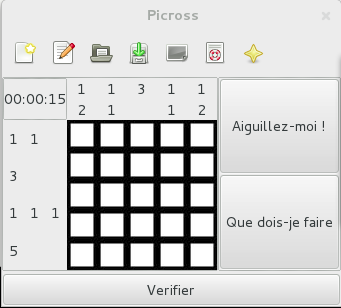
\includegraphics[scale=0.6]{data/screenMaquette/plateau.png}\\
                      \textbf{  plateau du jeu}\\
                      \end{center}
              

        \subsection{Bouton Nouvelle Grille}
        
        \paragraph*{}
        possibilité de choisir une grille de jeu, de taille 5 par 5 cases, 10 par 10, 15 par 15, 20 par 20 ou enfin 25 par 25. La difficulté est croissante avec la taille du jeu.
        
        \begin{center}
                      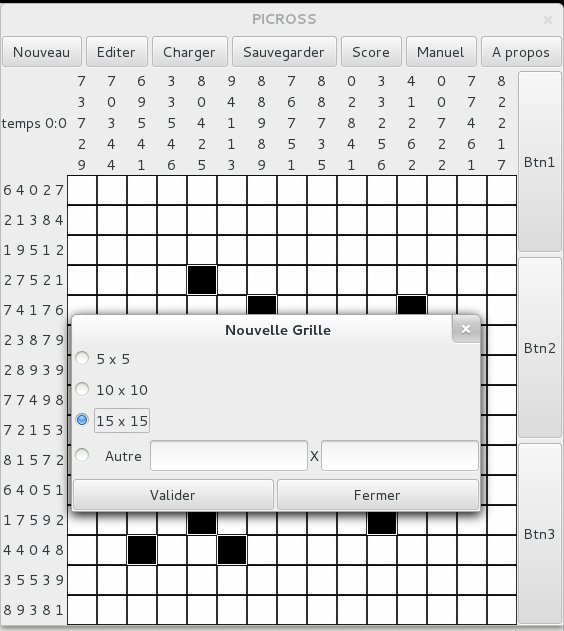
\includegraphics[scale=0.6]{data/screenMaquette/NouvelleGrille.png}\\
                      \textbf{Picross Grille}
        \end{center}
        

         
        
        \subsection{Bouton Sauvegarde}      
              \paragraph*{}
              Ce bouton permet de sauvegarder l'avancement de la grille actuelle.
              
              \begin{center}
                      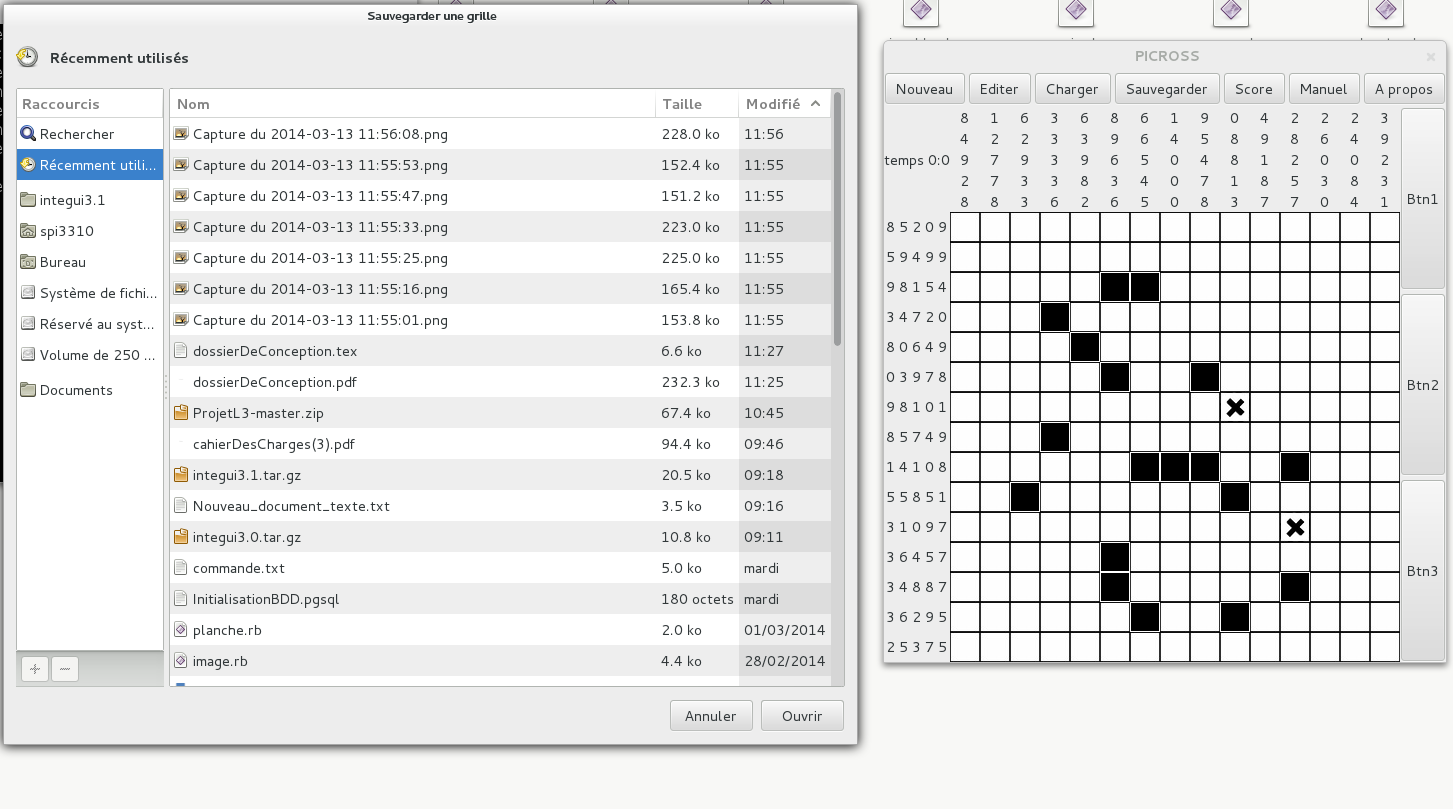
\includegraphics[scale=0.6]{data/screenMaquette/SauvegardeGrille.png}\\
                      \textbf{ Picross Grille Sauvegarde}
              \end{center}


        \subsection{Bouton Score :}
               Il donne, pour chacun des meilleurs scores, le temps passé sur la grille et le nombre d'appel à l'aide. Le nom de profil du joueur ayant réalisé le score est également affiché.
            
            
        \subsection{Manuel:}
              le Manuel est la fenêtre d’aide que l’on peut ouvrir via le menu. Il permettra d'ouvrir le manuel d'aide.\\ 
              
              
              
\section{Manuel d’instructions}
    \subsection{}
    \paragraph{}
    
      La grille générée par défaut est de la même taille que la grille abordée au dernier démarrage. Comme les développeurs sont très nuls au picross, une taille de 5 par 5 apparaîtra au premier lancement. Vous pouvez lancer une nouvelle partie en allant dans le menu Nouvelle Partie en choisissant la taille de la grille.\\      

      Remplissez la grille en s’aidant des informations placées horizontalement et verticalement. Elles correspondent au nombre de cases à noircir consécutivement\\
      
    Si vous trouvez une case correcte, celle-ci se grise. Si la case est incorrecte, c’est une erreur et une croix rouge se dessine.\\
      
      Si vous pensez avoir trouvé une case incorrecte, cochez-la à l’aide du clic droit. La case est sécurisée.\\
      
      Pour obtenir de l’aide, cliquez sur les boutons "Aiguillez-moi!" ou "Que dois-je faire ?". 
      Un conseil vous sera donné en dessous de la grille. Un aiguillage restera vague, et "Que dois-je faire ?" vous donnera un indice très précis. 
      Néanmoins, un appel à l'aide plus précise augmentera de 2 et non de 1 le nombre d'appel à l'aide dans vos scores.\\




\end{document}
% END
